\documentclass{article}

\usepackage{graphicx}
\graphicspath{{figs/}}

\author{Sean Finch and Chris Pollard}
\date{2012 12 13}
\title{Nonlinear Analysis of Elementary Cellular Automata}

\begin{document}
\maketitle

\vspace{0.5in}

\begin{figure}[h!]
    \centering
    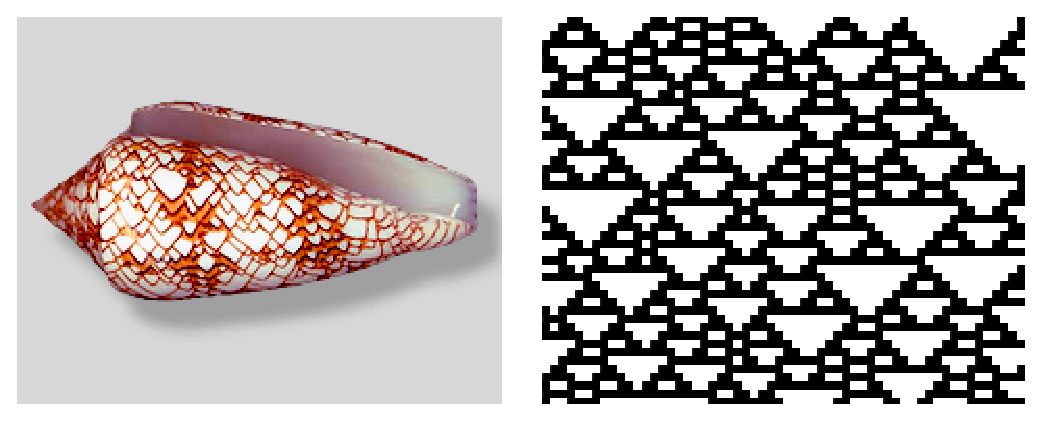
\includegraphics[width=\textwidth]{shell-automata.eps}
\end{figure}

\vspace{0.5in}

\begin{abstract}
    We present an introduction to and analysis of Elementary Cellular
    Automata (ECAs) as defined in Stephen Wolfram's
    \emph{A New Kind of Science}~\cite{anks}.
    ECAs are inherently nonlinear and their time evolution can
    exhibit extremely complex behavior--an unexpected feature given
    that their dynamics are governed by completely deterministic
    rules.
    This report demonstrates a simple analysis of several ECAs in the
    context of nonlinear systems.
\end{abstract}

\newpage

\section{Introduction}

% TODO
See the awesome Figure~\ref{110_map}.

Something about nonlinear dynamics in general and how discrete
nonlinear systems can display complexity with a small number of
parameters--e.g. logistic map.

\subsection{Elementary Cellular Automata}
% TODO

An Elementary Cellular Automaton (ECA) is defined in Stephen Wolfram's
\emph{A New Kind of Science}~\cite{anks}

\subsection{Automata Rules}
% TODO
- Rules and rule numbering

\subsection{Examples}
% TODO
- Examples (many figures)

% TODO
\begin{figure}
    \centering
    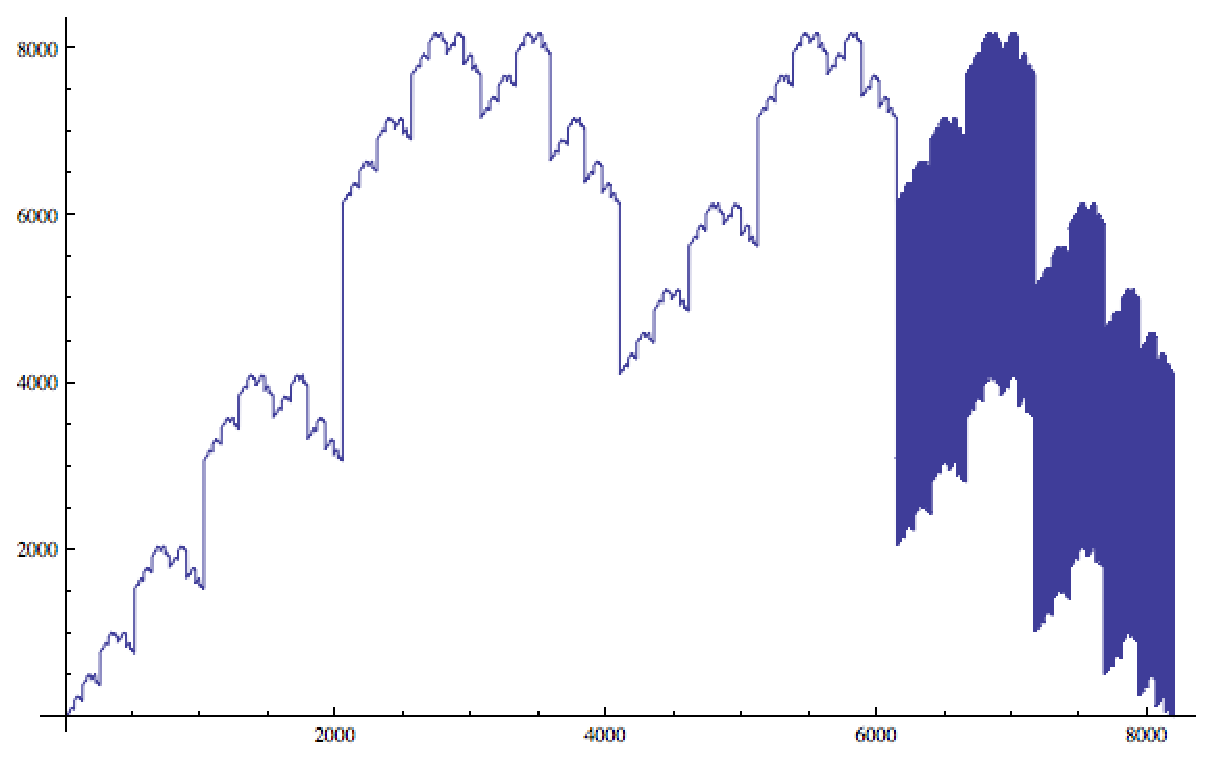
\includegraphics[width=0.49\textwidth]{110_13.eps}
    \caption{\label{110_map} Fractal map for rule 110 and a 13-site grid.}
\end{figure}

\begin{figure}
    \begin{minipage}[b]{0.49\textwidth}
        \centering
        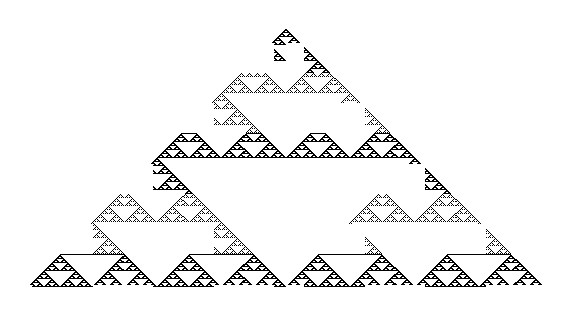
\includegraphics[width=\textwidth]{rule126.eps}
        \caption{\label{rule126} Rule 126}
    \end{minipage}
    \hspace{0.5cm}
    \begin{minipage}[b]{0.49\textwidth}
        \centering
        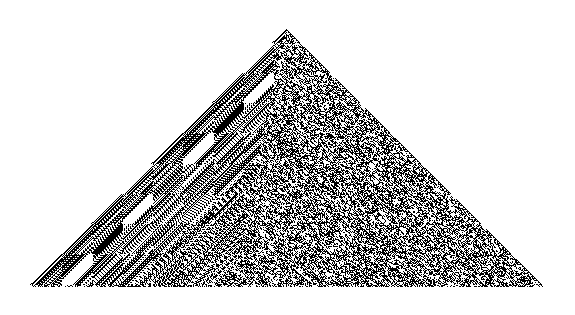
\includegraphics[width=\textwidth]{rule30.eps}
        \caption{\label{rule30} Rule 30}
    \end{minipage}
\end{figure}


\begin{figure}
    \begin{minipage}[b]{0.49\textwidth}
        \centering
        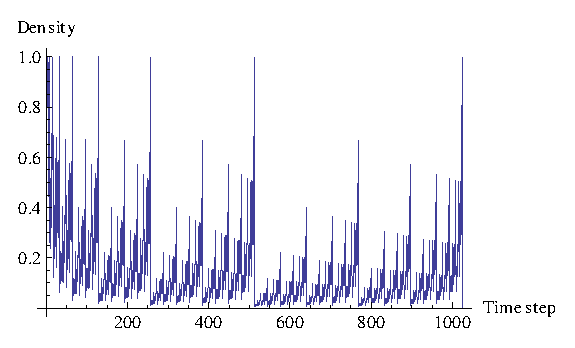
\includegraphics[width=\textwidth]{126density.eps}
        \caption{\label{126density} The Density of rule 126 plotted as a function of time step}
    \end{minipage}
    \hspace{0.5cm}
    \begin{minipage}[b]{0.49\textwidth}
        \centering
        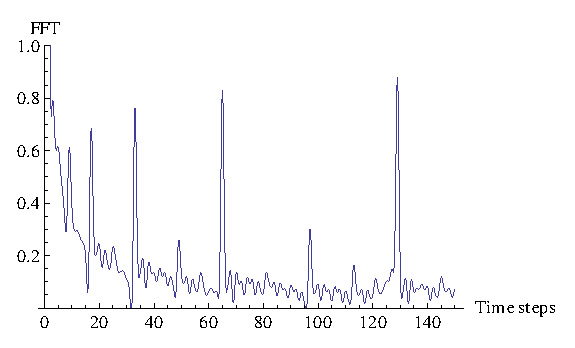
\includegraphics[width=\textwidth]{126FFT.eps}
        \caption{\label{126FFT} The FFT of rule 126's density, showing sharp peaks at 2$^n$.}
    \end{minipage}
\end{figure}


\begin{figure}
    \begin{minipage}[b]{0.49\textwidth}
        \centering
        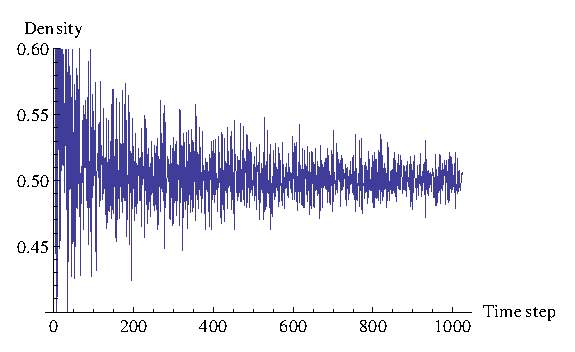
\includegraphics[width=\textwidth]{30density.eps}
        \caption{\label{30density} The Density of rule 30 plotted as a function of time step}
    \end{minipage}
    \hspace{0.5cm}
    \begin{minipage}[b]{0.49\textwidth}
        \centering
        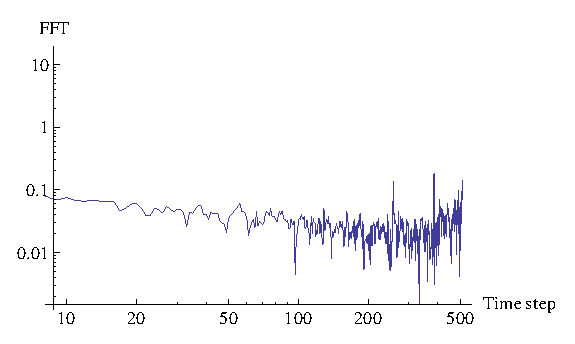
\includegraphics[width=\textwidth]{30FFT.eps}
        \caption{\label{30FFT} The FFT of rule 30's density.  The flat transform is the same as white noise.}
    \end{minipage}
\end{figure}

\section{Analysis of a Simple System Observable}

An Elementary Cellular Automaton with $n$ sites per time step has
$n$ degrees of freedom.
As one studies ECAs with larger $n$ values, it becomes a daunting
task to track the state of each individual site at each time step, and
an analysis of the time evolution of the system as a whole becomes
more meaningful.
In order to study the general behavior of the ECA systems, we wanted
to define an observable which collapsed these $n$ degrees of freedom
into one number whose value could be tracked over many time steps.
However, there are only so many such variables for such simple
systems value is meaningful for a wide variety of initial conditions
and boundary condition constraints.


\subsection{Defining an Observable}

We chose to study the density of black blocks as a convenient
observable for collapsing the information encoded in an $n$-site ECA
into one value per time step.
For ECAs with periodic or fixed boundary conditions, the density of
black blocks is straightforward:

\begin{equation}
    \rho = \frac{n_{black}}{n},
\end{equation}

\noindent where $n$ is the number of sites in the ECA.

One must be careful in the case of ECAs without boundary conditions
because the extent of the ECA is essentially infinite, and the above
definition of the black block density is not well-defined.
However, because the ECA rules only allow the state of a block to
depend on the previous states of its immediate neighbors, we chose
an initial condition of one black block surrounded by an infinite
number of white blocks on either side and constrained our studies to
rules which allow black blocks to spread by only one site per time
step.
Under these conditions there can be no black blocks outside of the
triangle with width $w(t)$ defined by $w(t) = 2t+1$, where $t$ is the
number of time steps since the initial state.
Treating $2t+1$ as the effective size of the Cellular Automaton at a
given time, the density of black blocks can be redefined as

\begin{equation}
    \rho = \frac{n_{black}}{(2t+1)}.
\end{equation}

\subsection{Density Time Evolution}
For ECAs with periodic or fixed boundary conditions, there is a
maximum number of global states available to the system: if there are
$n$ sites and each must have a value of 0 or 1, there will be $2^n$
possible states.
As such, after at most $2^n$ time steps the system must return to
a state that it has visited previously, and of course the density as a
function of time will be periodic.

However, ECAs with no boundaries have access to an infinite number of
states and therefore can exhibit a much richer density spectrum.
Any observed periodic behavior is significant because the system is
not confined to a finite number of states, and periodicity in the
density can only come about due to the intrinsic properties of a
particular rule.
Because of this, we have chosen to present the density's time
evolution for infinite ECAs.

Clearly not all ECA rules are created equally, and several of them are
not suitable for a study such as this.
For instance, with an initial state of one black block the Cellular
Automaton governed by rule 254 (Figure~\ref{rule254}) yields a string
of black blocks with width $2t+1$ at time step $t$.
This ECA will have a constant black block density of 1 given the above
definition.
However, most rules yield an interesting time evolution.
We will focus on the two rules mentioned previously, one (rule 126) of which is
very clearly periodic and has a well-defined structure and one (rule
30) whose dynamics appear to be random and incoherent.
The density as a function of time for rule 126 can be found in
Figure~\ref{126density}; that for rule 30 can be found in
Figure~\ref{30density}.


\begin{figure}
    \begin{minipage}[b]{0.49\textwidth}
        \centering
        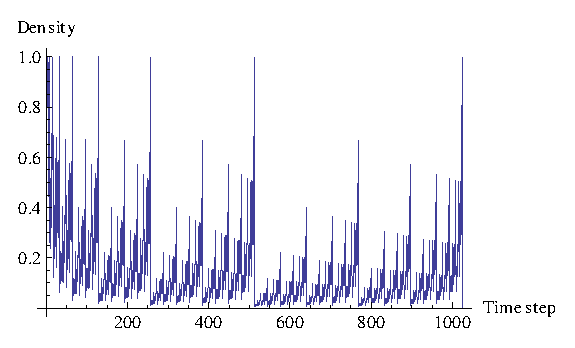
\includegraphics[width=\textwidth]{126density.eps}
        \caption{\label{126density} The black block density of rule 126 plotted as a function of time step}
    \end{minipage}
    \hspace{0.5cm}
    \begin{minipage}[b]{0.49\textwidth}
        \centering
        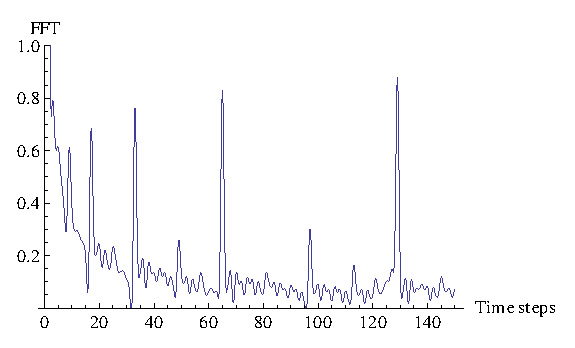
\includegraphics[width=\textwidth]{126FFT.eps}
        \caption{\label{126FFT} The Fast Fourier Transform (FFT) of
        rule 126's black block density, showing sharp peaks at 2$^n$}
    \end{minipage}
\end{figure}


\begin{figure}
    \begin{minipage}[b]{0.49\textwidth}
        \centering
        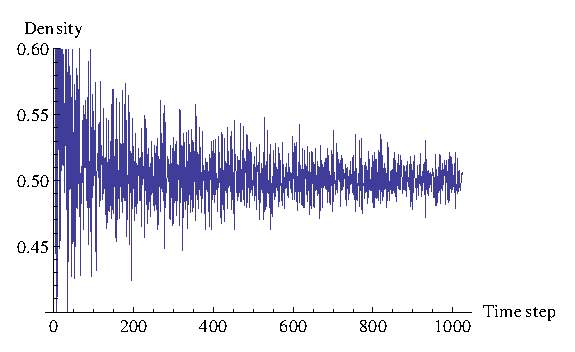
\includegraphics[width=\textwidth]{30density.eps}
        \caption{\label{30density} The black block density of rule 30 plotted as a function of time step}
    \end{minipage}
    \hspace{0.5cm}
    \begin{minipage}[b]{0.49\textwidth}
        \centering
        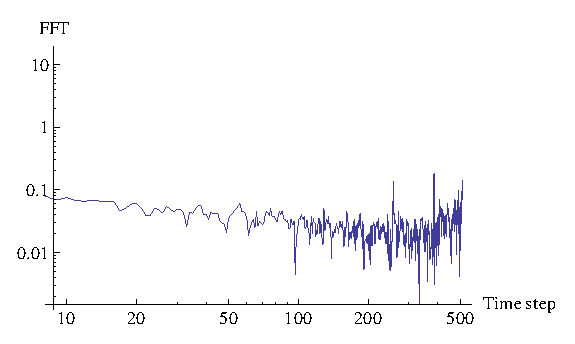
\includegraphics[width=\textwidth]{30FFT.eps}
        \caption{\label{30FFT} The FFT of rule 30's black block density}
    \end{minipage}
\end{figure}


\subsection{Periodic Density Analysis}
In order to establish whether or not an ECA's black block density
exhibits periodicity, we chose to look at its Discrete Fourier
Transform (DFT), specifically the Fast Fourier Transform (FFT), as
well as its Autocorrelation.

The DFT of a sequence of values is defined as

\begin{equation}
    \rho_p = \sum_{t=0}^{T-1} \rho_t e^{-2\pi i pt/T} \qquad p =
    0, 1,\ \ldots\ T,
\end{equation}

\noindent where $\rho_t$ is the black block density at a time step
$t$, $T$ is the total number of time steps, and $p$ is an integer
value of time steps which labels the discrete frequency
$\omega_p = p/T$.
Values of $p$ with a high coefficient $\rho_p$ correspond to strong
sinusoidal motion with a frequency of $\omega_p$.

From Figure~\ref{126FFT} we can see that rule 126 has clear sinusoidal
behavior, especially for values of $p$ that are a power of 2 ($2^n$
with integer n).
This is not terribly surprising given the structure of the ECA under
rule 126 in Figure~\ref{rule126}.

However, Figure~\ref{30FFT} shows that the opposite is true for rule
30.
In fact, the density FFT for rule 30 closely resembles that of random
noise, which should have a flat response as a function of frequency.

Similarly, the Autocorrelation function of a sequence of real values
is given by

\begin{equation}
    C_\tau = \frac{1}{T}\sum_{t=0}^{T-1} \rho_t \ \rho_{t-\tau} \qquad
    \tau = 0, 1,\ \ldots\ T,
\end{equation}

\noindent where $\rho_t$ is the black block density at a time step
$t$, $T$ is the total number of time steps, and $\tau$ is an integer
value of separation in time.
A high coefficient $C_\tau$ corresponds to a time separation for which
the density of black blocks is strongly correlated.
For example, a large value of $C_5$ would suggest that densities
separated by 5 time steps tend to have approximately the same value,
while a coefficient close to zero implies that they fluctuate randomly
around the mean.
If they are anticorrelated, we would see a negative autocorrelation
coefficient.

\begin{figure}
    \begin{minipage}[b]{0.49\textwidth}
        \centering
        \includegraphics[width=\textwidth]{126corr.eps}
        \caption{\label{126corr} The black block density's
        Autocorrelation for a rule 126 ECA.}
    \end{minipage}
    \hspace{0.5cm}
    \begin{minipage}[b]{0.49\textwidth}
        \centering
        \includegraphics[width=\textwidth]{30corr.eps}
        \caption{\label{30corr} The black block density's
        Autocorrelation for a rule 30 ECA.}
    \end{minipage}
\end{figure}

Figure~\ref{126corr} shows that there is a strong correlation between
densities separated by a time period equal to a power of 2 ($2^n$
with integer n).
Again, this is not unexpected given the structure rule 126 imposes and
the sinusoidal features expressed in its DFT.

Figure~\ref{30corr}, however, has some very interesting features which
lend a little more insight to rule 30 than its density DFT.
Despite what appears to be random behavior, there clear correlations
between densities separated by 8 time steps.
This is in part be due to the quasi-periodic behavior of the left
half of rule 30's ECA (see Figure~\ref{rule30}).
However, the fact that this correlation is also present for time
separations that are multiples of 8 suggests that its right half
(which seems to be without structure) is not as random as at first
glance.

\section{ECA as Discrete Maps}

As shown in section 2, ECA that are allowed to grow infinitely in size can exhibit non-periodic and chaotic behavior, even though they are completely deterministic.   
In this section we will only consider CA with a fixed number of cells.  
For this case, we must apply either fixed or periodic boundary conditions on the endpoints.  
In this work we use periodic boundary conditions and the phase space morphs from an infinite 1D lattice into a finite circular lattice.  
For an ECA of finite width, n, there exists $2^n$ possible configurations (each site takes one of two values).  
This means that every initial condition will eventually end in a periodic loop, although the period could be as large as $2^n -1$.  

\subsection{Converting rules into maps}

We follow the methods of~\cite{sed} to convert the graphical ECA rules into discrete 1D maps.  
In the same way each rule is labeled by a binary number, each time step in our finite ECA may be converted from binary into a base-10 number.  
We wrote a \textsc{C++} code to loop over all $2^n$ possible configurations and record the resulting configuration after one time step (both are recoded in base 10).  
Compiling all this information together, we get a 1D discrete map, mapping all the integers [0, $2^n -1$] $\rightarrow$ [0, $2^n -1$] for a given ECA rule.  
The resulting maps are shown in Figures~\ref{30map} and~\ref{126map}.  
The densely filled area is a result of lines connecting all successive points in the map.  
Figure~\ref{30map_dot} shows the same figure without the  lines connecting successive points.  
We can now iterate this mapping, using either cobweb diagrams or computer routines, to see the evolution of ECA over each time step.  

\begin{figure}
    \begin{minipage}[b]{0.49\textwidth}
        \centering
        \includegraphics[width=\textwidth]{30map.eps}
        \caption{\label{30map} The mapping for rule 30, using a grid width of 10 lattice points.  }
    \end{minipage}
    \hspace{0.5cm}
    \begin{minipage}[b]{0.49\textwidth}
        \centering
        \includegraphics[width=\textwidth]{30map_dot.eps}
        \caption{\label{30map_dot} Figure~\ref{30map}, shown without lines connecting successive points.}
    \end{minipage}
\end{figure}

The resulting maps are much more complicated in appearance than any of the maps we studied during the semester, such as the chaotic logistic map.  
The maps studied here have descrete values along the axes, where as the logistic map is continuous, so there is no possibility of rounding error or computer dependent results.  
Adding more lattice points to the map results in the same structure, but with a higher resolution.  
This is shown in Figures~\ref{126map_6} and~\ref{126map} where the lattice size is varied from six to ten points.  
Figure~\ref{126map_6} illustrates how rapid oscillations between two values leads to the filled in region.  
The two values differ by 512, or one bit, and demonstrate how changing one bit can lead to a very different response.   

\begin{figure}
    \begin{minipage}[b]{0.49\textwidth}
        \centering
        \includegraphics[width=\textwidth]{126map_6.eps}
        \caption{\label{126map} The mapping for rule 126 using a width of 6 lattice points.  }
    \end{minipage}
    \hspace{0.5cm}
    \begin{minipage}[b]{0.49\textwidth}
        \centering
        \includegraphics[width=\textwidth]{126map.eps}
        \caption{\label{126map_dot} The mapping for rule 126 using a width of 10 lattice points.}
    \end{minipage}
\end{figure}

\subsection{Dependence on Initial Conditions}

By iterating these maps we can look at the growth of the system as a function of time step.  As previously mentioned, all initial conditions will eventually reach a periodic cycle.  Figure~\ref{30iter_IC32} shows the growth of rule 30 over 1,000 iterations with initial condition 32 (one black block).  This system hits a stable period-15 cycle after 7 iterations.  Figure~\ref{30iter_IC33} shows the same evolution of rule 30, but now with initial condition 33.  These two initial conditions only differ by one bock, but the system now hits a period-5 cycle immediately after starting.  

Figure~\ref{30iter_IC34} once again shows rule 30 over 1,000 time steps, now with an initial value of 34.  Bit wise, the initial condition of 34 differs by only one cell from 32, and has two adjacent cells swapped from 33.  We can see that the initial value 34 takes slightly longer (25 iterations) but also settles on a period-15 cycle.  This period-15 cycle, however, is completely different from the period-15 cycle produced by starting condition 32.  Even though the initial conditions may not be continuously varied in these discrete systems, a strong sensitivity to initial conditions is still present.  

\begin{figure}
    \begin{minipage}[b]{0.49\textwidth}
        \centering
        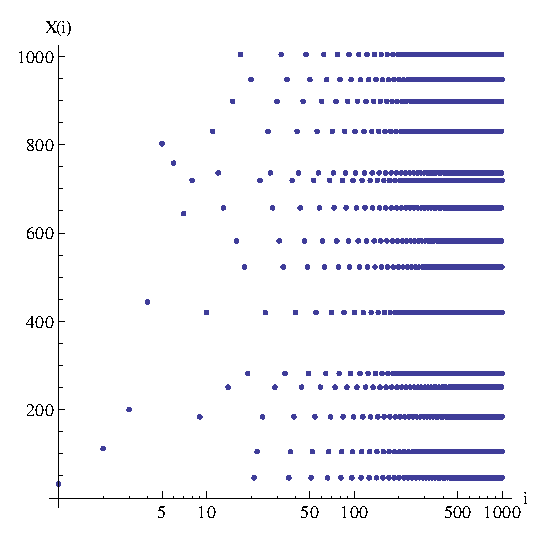
\includegraphics[width=\textwidth]{30iter_IC32.eps}
        \caption{\label{30iter_IC32} 1,000 iterations of rule 30 with an initial value of 32.   }
    \end{minipage}
    \hspace{0.5cm}
    \begin{minipage}[b]{0.49\textwidth}
        \centering
        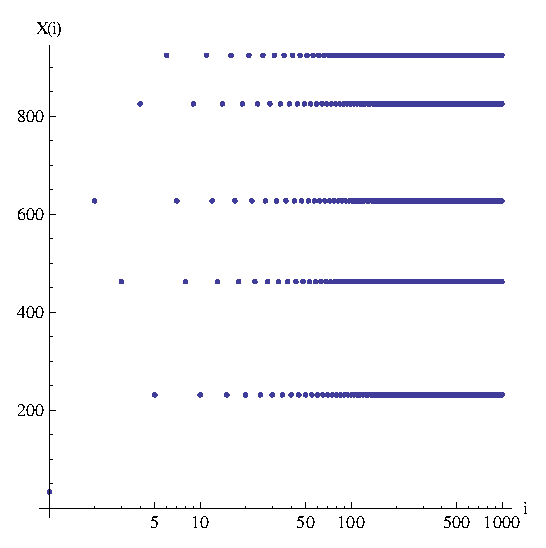
\includegraphics[width=\textwidth]{30iter_IC33.eps}
        \caption{\label{30iter_IC33} 1,000 iterations of rule 30 using the initial value 33. }
    \end{minipage}
\end{figure}

\begin{figure}
    \begin{minipage}[b]{0.49\textwidth}
        \centering
        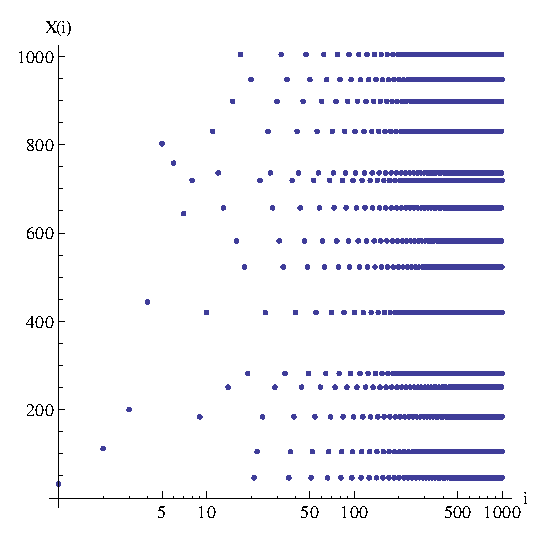
\includegraphics[width=\textwidth]{30iter_IC32.eps}
        \caption{\label{30iter_IC32_2} 1,000 iterations of rule 30 with an initial value of 32.   }
    \end{minipage}
    \hspace{0.5cm}
    \begin{minipage}[b]{0.49\textwidth}
        \centering
        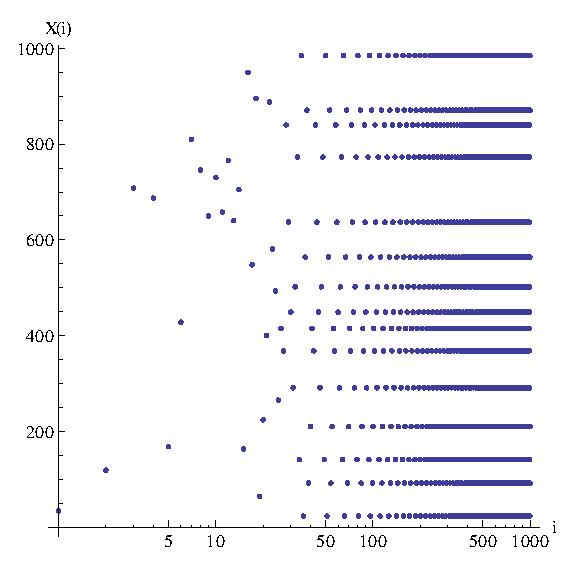
\includegraphics[width=\textwidth]{30iter_IC34.eps}
        \caption{\label{30iter_IC34} 1,000 iterations of rule 30 using the initial value 34. }
    \end{minipage}
\end{figure}

We can run our code for all initial values from 0 to $2^n$ and plot the resulting limit cycle.  This information is plotted in Figure~\ref{30bif} for rule 30 and Figure~\ref{126bif} for rule 126.  From these plots it can be seen that there is a high variability in which limit cycle results from different initial conditions.  There is an interesting trend where bands of states do not appear in any of the possible limit cycles.  

\begin{figure}
    \begin{minipage}[b]{0.49\textwidth}
        \centering
        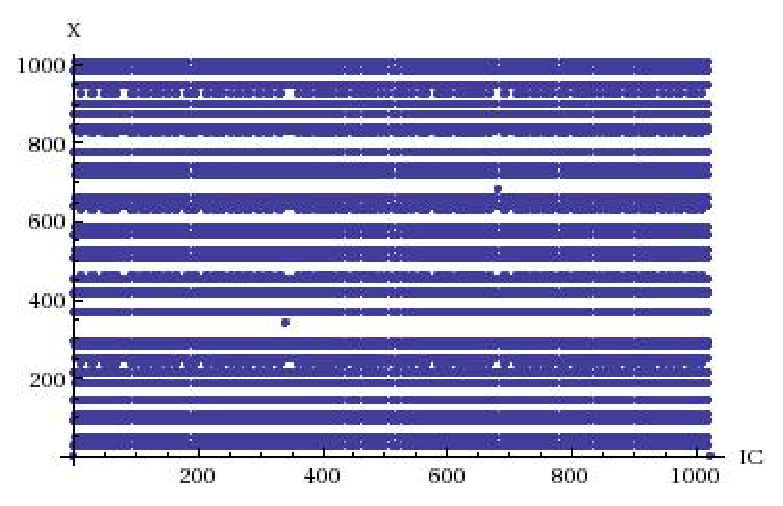
\includegraphics[width=\textwidth]{30bif.eps}
        \caption{\label{30bif} The limit cycles of rule 30, plotted as a function of all initial conditions [0, 1023]}
    \end{minipage}
    \hspace{0.5cm}
    \begin{minipage}[b]{0.49\textwidth}
        \centering
        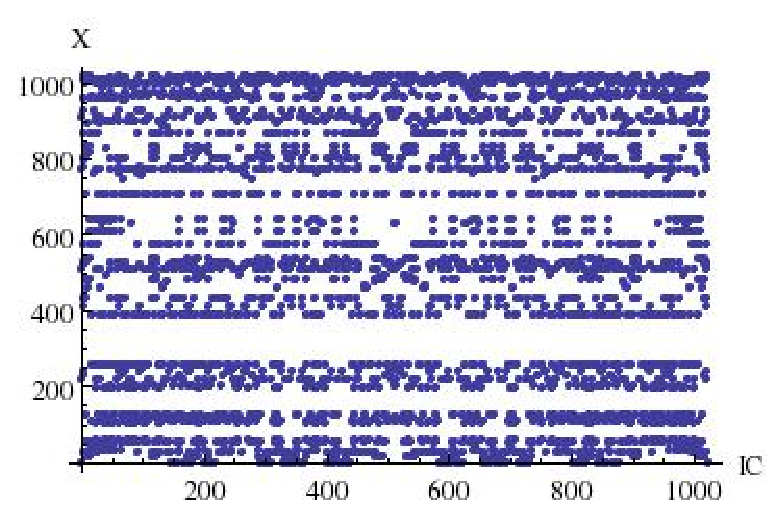
\includegraphics[width=\textwidth]{126bif.eps}
        \caption{\label{126bif} The limit cycles of rule 126, plotted as a function of all initial conditions [0, 1023] }
    \end{minipage}
\end{figure}

\subsection{Fractal Dimension}

Many of the ECA rules result in fractal patterns.  The easiest way to classify these patters is by their fractal dimension.  The fractal dimension is given by:
\begin{equation}
	D = - \frac{log N}{log \epsilon},
\end{equation}
where N is the number of new branches per iteration and $\epsilon$ is the scaling factor for each branch.  The fractal image produced by rule 126, shown in Figure~\ref{rule126}, has N = 3 branches per iteration and a scaling factor of $\epsilon$ = 0.5.  This results in a fractal dimension of $log 3/log 2 \approx 1.58$.  Interestingly, the map version of rule 126 also shows repeating shapes with a scaling factor of 0.5 and, although hard to see, three branches per iteration.  This would give the map the exact same fractal dimension as the Sierpinski triangle pattern that it creates.  It should be noted that this argument is only valid as the number of lattice points goes to infinity, the map is one dimensional for a finitely sized lattice.  




\section{Conclusion}

ECA show the remarkable property that simple, completely deterministic rules can lead to complex and chaotic behavior.  

\subsection{Application in Cryptography}

One possible application of ECA is cryptography.  Cryptography relies on having an encrypting function that is easy to computationally compute in one direction, but inverse is extremely computationally intensive without knowledge of the key.  ECA fits this description: a binary sequence my be encrypted by applying an ECA rule and iterating over several time steps.  Determining the inverse is much harder since each cell is not uniquely determined, but depends on its also undermined neighbor.  Furthermore, the sensitivity to initial conditions implies that a one bit error in decoding the message will affect the entire message after many iterations.  To efficiently decode the message, one would use a key containing additional information, such as the ECA rule used, the format of initial conditions, and number of iterations.  The inverse of ECA then becomes solvable on a reasonable time scale.  



\bibliographystyle{plain}
\bibliography{bib}

\appendix
\section{Code}

\begin{verbatim}

n = 1024;
m = CellularAutomaton[126, {{1}, 0}, n];
sumBlacks = Total[m, {2}]; 
Do[
  sumBlacks[[i]] = sumBlacks[[i]]/(2*(i - 1) + 1)
  , {i, 1, n + 1}
]

ArrayPlot[m, Frame->False]
ListLinePlot[sumBlacks, PlotRange -> All, 
  AxesLabel -> {"Time step", "Density"}]
ListLinePlot[Abs[Take[Fourier[sumBlacks], 150]],  PlotRange -> {0, 1},
  InterpolationOrder -> 2, AxesLabel -> {"Time steps", "FFT"}]


\end{verbatim}


\end{document}
